% PSM: Probabilistic Spatial Memory for Wearable Look-Back QA
% All sections compressed for 14-page ECCV LNCS limit (v2, 2026-06-22).
%
% Build: pdflatex main && bibtex main && pdflatex main && pdflatex main
% Kit files (eccv.sty, eccvabbrv.sty, llncs.cls, splncs04.bst,
% eijkel2.{eps,pdf}) are vendored into this directory so any fresh
% clone can build without re-cloning the upstream ECCV template.
%
% TODO REVIEW: replace ID=***** with the OpenReview submission ID
% TODO FINAL : swap `\usepackage[review,...]{eccv}` for `\usepackage{eccv}`
%              and the pagebackref hyperref line below.

\documentclass[runningheads]{llncs}

% ECCV 2026 author-kit package (rides on top of llncs.cls).
% The `review` option enables line numbering + paper-ID watermark.
\usepackage[review,year=2026,ID=*****]{eccv}
% ECCV-standard abbreviation macros (\eg, \ie, \etc, \cf, \etal).
\usepackage{eccvabbrv}

% Body packages. Keep this list short; the kit forbids any package
% that alters layout (textheight, vspace, baselinestretch, etc.).
% eccv.sty already loads: fontenc[T1], amsmath, amssymb, xcolor[dvipsnames],
% cite, xspace, url[hyphens], lineno, caption, subcaption — don't re-load.
\usepackage[utf8]{inputenc}
\usepackage{microtype}
\usepackage{graphicx}
% Figure PDFs (F2/F3/F6/F7) are generated in journal/figures/ by
% scripts/plot_f*.py; symlinks in paper_drafts/figures/ point there
% so \includegraphics{figures/...} resolves without \graphicspath.
\usepackage{booktabs}
% Accessibility tagging — required by the ECCV 2026 author kit.
\usepackage[accsupp]{axessibility}
\usepackage{pifont}
\usepackage{tikz}
\usetikzlibrary{positioning, arrows.meta, fit, calc,
                shapes.geometric, backgrounds}

% Hyperref — review version uses pagebackref so reviewers can jump
% from a bibliography entry back to citing pages.
% TODO FINAL: swap for plain `\usepackage{hyperref}` in camera-ready.
\usepackage[pagebackref,breaklinks,colorlinks,citecolor=eccvblue]{hyperref}

% Macros used across sections.
\newcommand{\psm}{\textsc{PSM}\xspace}
\newcommand{\caponek}{\texttt{per\_cell\_cap}\xspace}
% Per-cell PASS / FAIL marks for the multi-corpus acceptance table.
% pifont's \ding chars match the LNCS body font weight better than
% amssymb \checkmark / $\times$ at the cell sizes used in tables.
\newcommand{\cmark}{\ding{51}}
\newcommand{\xmark}{\ding{55}}

\title{Probabilistic Spatial Memory: A Bounded-Memory Retrieval
Substrate for Wearable Look-Back Question Answering}
\titlerunning{Probabilistic Spatial Memory for Wearable Look-Back QA}

% TODO FINAL: replace Anonymous block with author list + ORCIDs.
\author{Anonymous}
\authorrunning{Anonymous}
\institute{Anonymous Institution\\\email{anon@example.com}}

\begin{document}

\maketitle

\begin{abstract}
For an agent to hold persistent memory of its environment, its state
cannot grow unboundedly with observation time. We propose
\textbf{Probabilistic Spatial Memory} (\psm), a \emph{dynamic spatial
representation} whose state is budgeted by physical area explored rather
than by sequence length. \psm{} is a streaming spatial-temporal index
combining an H3 hex-grid tessellation, a time-decayed ring buffer of
HyperLogLog sketches per cell for \emph{test-time memory updating}, and
reservoir-sampled embedding exemplars. It exposes a novel \caponek{} knob
that smoothly trades strict spatial diversity for embedding-similarity
precision---dialing state size against recall in the spirit of the
recall--throughput tradeoff studied for sequence
models~\cite{arora2024linear,chen2024vljepa}.

We evaluate \psm{} as a retrieval substrate on egocentric look-back QA
(``where did I leave my keys?''), where memory-budgeted operation is a
hard constraint. At the bounded deployment point ($R{=}128$,
\texttt{cap}=$K$), \psm{} reaches 21/187 Hit@5 on the Nymeria proxy
session vs.\ brute-force CLIP's 25/187, at $8\times$ smaller,
session-length-invariant per-cell state. With reservoir eviction removed
($R{=}1024$), the same endpoint recovers the identical 25/187 hit set,
a substrate-correctness check confirming the expected top-$K$ equivalence.
The spatial-axis discrimination generalizes across \textbf{14 street-scale
sessions} drawn from \textbf{3 distinct sensor stacks} (SLOPER4D
head-mounted LiDAR, Nymeria + LookOut~\cite{pan2025lookout} Project
Aria MPS) and \textbf{3 encoder families} (laion CLIP-L / CLIP-bigG,
Google SigLIP~2~\cite{tschannen2025siglip2}): 13/14 sessions pass a
monotone-r10$\to$r12 Hit\,@\,5 acceptance with $\geq 4$\,pp lift on
at least one encoder. Because \psm{} retrieves candidates from
query-matched H3 cells rather than uniform time slices, it supplies the
spatial-temporal prefilter that frontier MLLMs lack: on four of these
sessions, uniform $K{=}8$ sampling yields Hit\,@\,5 $= 0\%$---the MLLM
never sees a ground-truth frame, regardless of its reasoning capability,
and \psm{}'s cell-targeted retrieval removes this structural blind spot.
The C engine ($\sim$700 LoC) and Python eval harness are released
under MIT.

\keywords{Spatial memory \and Bounded memory \and Dynamic spatial
representation \and Test-time memory updating \and Probabilistic data
structures \and Egocentric video \and Retrieval substrate.}
\end{abstract}

% ---- Body sections -------------------------------------------------
% Section 1 — Introduction
% Status: v1 draft. Anchor on Wearables AI CFP topic-area alignment
% and the three-paragraph contribution structure:
%   (1) The problem: streaming egocentric retrieval is unbounded;
%       brute-force CLIP grows linearly in N.
%   (2) The architecture: PSM as a spatial-temporal index +
%       reservoir-sampled exemplars + ring-buffer time decay, with
%       per_cell_cap as the tuneable place-vs-similarity knob.
%   (3) The contribution: bounded PSM approaches brute-force while the
%       full-reservoir row checks the expected cap=K equivalence.

\section{Introduction}
\label{sec:intro}

For an intelligent agent to hold persistent memory of its environment, its internal state cannot grow unboundedly with time. Standard retrieval-augmented systems embed every observation into a dense vector bank that grows linearly with recording duration, making continuous multi-session memory prohibitively expensive on-device. Long-context modeling of the models themselves~\cite{arora2024linear} does not address the systems bottleneck: how to structure a dynamic spatial representation supporting test-time memory updating without unbounded state explosion?

\paragraph{The memory-centric systems question.}
Rather than claim a new memory bound, we ask an empirical allocation question:
\emph{under a fixed global exemplar budget $M$, how should a streaming agent
decide which observations to keep, and does allocating that budget across space
(rather than across time) preserve more of the experiences a later query will
need?} This isolates \emph{allocation} from encoder quality and from total
memory: every policy we compare keeps the same number of exemplars and returns
the same number of candidates, so differences reflect what each policy chooses
to retain. \psm{} is one point in this space; its per-cell state is bounded and
grows sublinearly in the frame count, but the number of occupied cells grows
with area, so \psm{} is budgeted per cell and is \emph{not} globally
memory-bounded (\S\ref{sec:method}).

% F1 — PSM architecture overview (two-row layout for LNCS single column).
% Top row: streaming input + PSM ingest (Stages 0–1).
% Bottom row: query retrieval + MLLM rerank (Stages 2–3).
% Pure TikZ; requires \usetikzlibrary{positioning,arrows.meta,fit,
% calc,shapes.geometric,backgrounds} loaded in main.tex.
\begin{figure}[t]
\centering
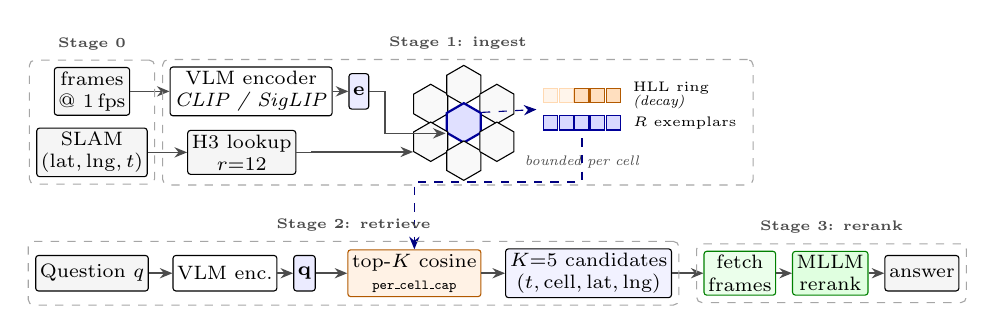
\begin{tikzpicture}[
    >={Stealth[length=1.6mm,width=1.3mm]},
    font=\scriptsize,
    node distance=1.5mm and 2mm,
    box/.style={draw, rounded corners=1pt, align=center,
                inner sep=1.5pt, minimum height=4.5mm, fill=white},
    iobox/.style={box, fill=gray!8},
    stage/.style={draw, dashed, rounded corners=2pt,
                  inner sep=2.5pt, gray!70},
    stagelbl/.style={font=\scriptsize\bfseries, gray!60!black},
    hex/.style={draw, regular polygon, regular polygon sides=6,
                minimum size=5mm, inner sep=0pt, rotate=30,
                fill=gray!5},
    hexhi/.style={hex, fill=blue!12, draw=blue!60!black, thick},
    hllbox/.style={draw, minimum width=1.8mm, minimum height=1.8mm,
                   inner sep=0pt, fill=orange!25, draw=orange!70!black},
    hllold/.style={hllbox, fill=orange!8, draw=orange!30},
    resvslot/.style={draw, minimum width=1.8mm, minimum height=1.8mm,
                     inner sep=0pt, fill=blue!15, draw=blue!60!black},
    flow/.style={->, semithick, gray!60!black},
    smallflow/.style={->, thin, gray!60!black},
]

% ===================== TOP ROW: Stages 0 + 1 =====================

% ---- Stage 0: streaming input ----
\node[iobox] (frames) {frames\\@ 1\,fps};
\node[iobox, below=1.5mm of frames] (slam) {SLAM\\$({\rm lat,lng},t)$};

% ---- Stage 1: PSM ingest ----
% Encoder
\node[box, right=5mm of frames] (enc) {VLM encoder\\\textit{CLIP / SigLIP}};
\node[box, right=2mm of enc, fill=blue!8] (emb) {$\mathbf{e}$};

% H3 lookup
\node[box, right=5mm of slam, fill=gray!8] (h3lookup) {H3 lookup\\$r{=}12$};

% H3 hex grid — compact 7-hex cluster
\coordinate (hexcenter) at ($(emb.east) + (12mm, -4mm)$);
\node[hex] (h0) at ($(hexcenter) + (-4.2mm, 2.4mm)$) {};
\node[hex] (h1) at ($(hexcenter) + ( 0mm,   4.8mm)$) {};
\node[hex] (h2) at ($(hexcenter) + ( 4.2mm, 2.4mm)$) {};
\node[hexhi] (hC) at (hexcenter) {};
\node[hex] (h4) at ($(hexcenter) + (-4.2mm,-2.4mm)$) {};
\node[hex] (h5) at ($(hexcenter) + ( 0mm,  -4.8mm)$) {};
\node[hex] (h6) at ($(hexcenter) + ( 4.2mm,-2.4mm)$) {};

% Per-cell state pop-out (right of hex grid)
\coordinate (cellAnchor) at ($(hexcenter) + (14mm, 0mm)$);

% Ring buffer of HLL sketches
\node[hllold]  (hll1) at ($(cellAnchor) + (-3.0mm, 3.5mm)$) {};
\node[hllold]  (hll2) at ($(cellAnchor) + (-1.0mm, 3.5mm)$) {};
\node[hllbox]  (hll3) at ($(cellAnchor) + ( 1.0mm, 3.5mm)$) {};
\node[hllbox]  (hll4) at ($(cellAnchor) + ( 3.0mm, 3.5mm)$) {};
\node[hllbox]  (hll5) at ($(cellAnchor) + ( 5.0mm, 3.5mm)$) {};
\node[font=\tiny, right=0.3mm of hll5, anchor=west, align=left]
     (hlllbl) {HLL ring\\[-0.5ex]\textit{(decay)}};

% Reservoir slots
\node[resvslot] (r1) at ($(cellAnchor) + (-3.0mm, 0mm)$) {};
\node[resvslot] (r2) at ($(cellAnchor) + (-1.0mm, 0mm)$) {};
\node[resvslot] (r3) at ($(cellAnchor) + ( 1.0mm, 0mm)$) {};
\node[resvslot] (r4) at ($(cellAnchor) + ( 3.0mm, 0mm)$) {};
\node[resvslot] (r5) at ($(cellAnchor) + ( 5.0mm, 0mm)$) {};
\node[font=\tiny, right=0.3mm of r5, anchor=west, align=left]
     (rsvlbl) {$R$ exemplars};

% Bounded label
\node[font=\tiny\itshape, below=2mm of r3, gray!60!black]
     (boundlbl) {bounded per cell};

% Connector from highlighted hex to pop-out
\draw[smallflow, dashed, blue!50!black]
     (hC.east) -- ($(hll1.west) + (-0.8mm, -1.8mm)$);

% Stage-0/1 flow arrows
\draw[flow] (frames.east) -- (enc.west);
\draw[flow] (enc.east)    -- (emb.west);
\draw[flow] (slam.east)   -- (h3lookup.west);
\draw[flow] (emb.east) -- ++(2mm,0) |- (hC.west);
\draw[flow] (h3lookup.east) -- ++(2mm,0) |- (h4.west);

% ===================== BOTTOM ROW: Stages 2 + 3 =====================

% Vertical offset below the ingest row
\coordinate (row2anchor) at ($(boundlbl.south) + (0, -6mm)$);

% ---- Stage 2: query ----
\node[iobox, align=center] (query)
    at ($(frames.south) + (0, -20mm)$)
    {Question $q$};
\node[box, right=3mm of query] (qenc) {VLM enc.};
\node[box, right=2mm of qenc, fill=blue!8] (qemb) {$\mathbf{q}$};

\node[box, right=4mm of qemb, align=center, fill=orange!10,
      draw=orange!70!black] (topk)
    {top-$K$ cosine\\{\tiny\texttt{per\_cell\_cap}}};

\node[box, right=3mm of topk, align=center, fill=blue!5] (cands)
    {$K{=}5$ candidates\\$(t,\text{cell},\text{lat},\text{lng})$};

% Flow: reservoir → top-K (vertical connector from row 1)
\draw[flow, dashed, blue!50!black]
    ($(r3.south) + (0, -1mm)$) -- ++(0, -5.5mm) -| (topk.north);

% Stage-2 flow arrows
\draw[flow] (query.east) -- (qenc.west);
\draw[flow] (qenc.east)  -- (qemb.west);
\draw[flow] (qemb.east)  -- (topk.west);
\draw[flow] (topk.east)  -- (cands.west);

% ---- Stage 3: MLLM rerank ----
\node[box, right=4mm of cands, align=center,
      fill=green!8, draw=green!50!black] (fetch)
    {fetch\\frames};
\node[box, right=2mm of fetch, align=center,
      fill=green!12, draw=green!50!black] (mllm)
    {MLLM\\rerank};
\node[iobox, right=2mm of mllm] (ans) {answer};

\draw[flow] (cands.east) -- (fetch.west);
\draw[flow] (fetch.east) -- (mllm.west);
\draw[flow] (mllm.east)  -- (ans.west);

% ===================== Stage bounding boxes =====================
\node[stage, fit=(frames)(slam),
      label={[stagelbl, anchor=south]above:{\tiny Stage 0}}] {};
\node[stage, fit=(enc)(emb)(h3lookup)(h0)(h2)(h5)(rsvlbl)(boundlbl),
      label={[stagelbl, anchor=south]above:{\tiny Stage 1: ingest}}] {};
\node[stage, fit=(query)(qenc)(qemb)(topk)(cands),
      label={[stagelbl, anchor=south]above:{\tiny Stage 2: retrieve}}] {};
\node[stage, fit=(fetch)(mllm)(ans),
      label={[stagelbl, anchor=south]above:{\tiny Stage 3: rerank}}] {};

\end{tikzpicture}
\caption{\textbf{PSM architecture.}
\emph{Top:} streaming frames are encoded and deposited into H3 cells;
each cell keeps a bounded ring of $C$ HLL sketches (orange, fading
with age) and $R$ reservoir-sampled embeddings (blue).
\emph{Bottom:} the query is encoded, cosine-searched against the
reservoirs with a \caponek{} gate, and the top-$K$ candidate frames
are reranked by a frontier MLLM.}
\label{fig:f1-architecture}
\end{figure}

Figure~\ref{fig:f1-architecture} sketches the end-to-end architecture.

\paragraph{Probabilistic Spatial Memory.}
We propose \textbf{\psm{}}, a streaming spatial-temporal index over an H3
hex-grid tessellation with three per-cell structures: reservoir-sampled
embedding exemplars; a time-decayed ring buffer of HyperLogLog sketches giving
per-cell cardinality and a temporal envelope; and a per-cell capacity bound
(\caponek{}) that dials strict spatial diversity ($\texttt{cap}{=}1$) to
unconstrained top-$K$ ($\texttt{cap}{=}K$). Ingestion is streaming and per-cell
state is bounded; query cost depends on scope (a spatially-centered query scans
only a k-ring of cells, while an uncentered query scans all retained exemplars).
We report engine ingest/query cost at the actual CLIP-L deployment
configuration in \S\ref{sec:results-memory-latency}; the CLIP encoder, not the
index, is the dominant on-device cost (\S\ref{sec:limitations}).

\paragraph{Evaluating the retrieval substrate.}
We evaluate \psm{} as a retrieval substrate on egocentric look-back QA (e.g., ``where did I last see my bike?'', ``when was I last at this intersection?''). Multimodal LLMs achieve strong single-frame grounding yet remain brittle on temporal grounding over long video~\cite{cheng2024videgothink,chen2025groundedmultihop}, so we compose \psm{} as an upstream spatial \emph{prefilter} to a frontier MLLM (\S\ref{sec:pipeline}): \psm{} supplies fixed-budget recall, the MLLM supplies localization precision.

\paragraph{Contributions.}
\begin{itemize}
  \item \textbf{A budget-matched allocation study.} On 14 street-scale
    egocentric sessions we compare streaming retention policies at an identical
    global exemplar budget and candidate count (global reservoir, FIFO,
    temporal stratification, a semantic $k$-center coreset, and a causal
    spatial-allocation probe), with rare/common-place and old/recent strata
    reported together (\S\ref{sec:results-main}).
  \item \textbf{A characterization, not a win.} Spatial allocation changes
    \emph{which} places are remembered, not aggregate retrieval: it helps
    rare/low-exposure-place recall in a \emph{place-specific} way (it beats
    coordinate-permutation nulls on 2/3 seeds and is robust to grid
    translation/rotation) but trades against common places, and a non-spatial
    semantic-diversity coreset is best overall. The spatial policy is an
    experimental probe with area-growing bookkeeping, not a deployed method.
  \item \textbf{\psm{} substrate + honest systems accounting.} A streaming H3
    index with per-cell reservoir exemplars and a time-decayed HLL ring
    (\S\ref{sec:method}); we report the engine's on-device cost at the actual
    CLIP-L deployment configuration and the corrected per-cell memory model on
    102.9\,h of driving (Honda HDD) as modeled logical state
    (\S\ref{sec:results-hdd}).
  \item \textbf{Correcting the MLLM framing.} A frontier-MLLM comparison shows
    query-aware retrieval beats uniform frame sampling; it does \emph{not} show
    that MLLMs require \psm{} (\S\ref{sec:results-vanilla-mllm}). Engine and
    budget-matched harness (policies, semantic/coordinate-null controls, paired
    statistics) are open-source under MIT.
\end{itemize}

% Section 2 — PSM architecture
% Status: v1 draft. Describes the engine's three data structures
% (H3 cells / ring buffer of HLLs / reservoir-sampled exemplars)
% and the per_cell_cap selection rule. Anchored on the actual
% C-side surface in include/core/{spatial_memory,tile,ring_buffer}.h
% so any future reader can navigate from the prose to the code.
% NB: former §3 (PSM-as-MLLM-prefilter pipeline) folded in as the final
% subsection, labelled sec:pipeline, during the 8pp cut.

\section{Probabilistic Spatial Memory}

\label{sec:method}

\psm{} is a streaming spatial-temporal index that ingests
$(t, \mathrm{lat}, \mathrm{lng}, \mathbf{e})$ tuples: timestamp,
geographic position, and a $d$-dimensional CLIP embedding. This supports
top-$K$ similarity search with capped per-cell state at any time. Three
components define the index.



\subsection{H3 spatial tessellation}
\label{sec:method-h3}

We tessellate the wearer's trajectory with H3~\cite{brodsky2018h3}, a
hierarchical hexagonal geospatial index. Each tuple maps to its containing cell
at resolution~$r$ (default~12, ${\sim}9$\,m edges, room scale; swept over
$r\in\{8,9,10,11,12\}$ in \S\ref{sec:results-multi-corpus}). H3 cell IDs are
global, comparable across recordings, sessions, and devices.
Positions come from whatever pose stream the device already runs: GNSS outdoors
(HDD's RTK fixes) or geo-anchored on-device SLAM/VIO indoors (Aria MPS,
LiDAR-SLAM); \psm{} needs only a consistent global frame, so the indoor ``keys''
setting uses the same localization the device already provides.

\subsection{Time-decayed ring buffer of HyperLogLog sketches}
\label{sec:method-ring-buffer}

Each cell maintains a ring buffer of $C$ HyperLogLog
sketches~\cite{flajolet2007hyperloglog} rotating on a time-window cadence
(default 30\,s): ingest hashes the embedding into the current sketch, and when
the window elapses the oldest sketch expires as the ring wraps. The sketches
give per-cell cardinality and expose the cell's \emph{temporal envelope}
$(t_{\min},t_{\max})$, returned as the bucket window the MLLM consumes as a
time-range hint. Each sketch is $2^p$ bytes ($p{=}10\Rightarrow$1\,KiB), so the
ring costs $C\cdot1\,\mathrm{KiB}=60\,\mathrm{KiB}$ at $C{=}60$ per cell,
independent of dwell time. What the sketch counts is the number of \emph{distinct
hashed embedding vectors}: for continuous CLIP embeddings, where near-duplicate
frames still differ in their raw bytes, this is close to the ingested frame count
rather than a count of semantically distinct events or objects. We therefore use
the cardinality as a cheap per-cell activity/temporal signal and \textbf{do not}
claim it counts ``unique events'' or ``distinct people'' without an upstream
object/event canonicalization stage (\S\ref{sec:limitations}). The HLL is thus
optional metadata unless it is wired to drive allocation, which we leave to future
work.

\subsection{Reservoir-sampled exemplars}
\label{sec:method-exemplars}

Counts and envelopes are not embeddings, so each cell also stores exemplars via
\emph{Algorithm~R reservoir sampling}~\cite{vitter1985reservoir} (capacity
$R{=}128$): after $n>R$ frames the reservoir holds a uniform random $R$-subset
(${\sim}0.38$\,MiB/cell at $R{=}128$, CLIP-L's $d{=}768$; ${\sim}0.44$\,MiB with
the HLL ring).

\paragraph{Memory profile (per-cell bounded, not globally bounded).} For a
trajectory visiting $C_n$ distinct H3 cells over $n$ frames, \psm{}'s state is
$\Theta\!\big(C_n(R d + C\,2^p)\big)$, whereas brute-force embedding storage is
$\Theta(n d)$. The \emph{per-cell} summary is bounded ($R$ exemplars plus a
$C$-slot HLL ring, independent of how long the wearer dwells), so state grows
sublinearly in $n$ \emph{when revisits dominate}: revisited and dwelled cells
saturate at $R$ rather than accumulating every frame. This is not a worst-case
bound independent of recording duration: $C_n$ grows with the physical area
explored, and under continual exploration $C_n=\Theta(n)$, so total state is
unbounded in the worst case. The HLL ring is charged to \emph{every} visited
cell, including the many single-visit ones, so on wide-area corpora it can
dominate the footprint (\S\ref{sec:results-hdd}). We therefore report exemplar
and ring bytes separately and, in \S\ref{sec:results}, study a \emph{fixed
global exemplar budget} that allocates a hard exemplar-payload ceiling across
cells; per-cell policy bookkeeping is reported separately.
Figure~\ref{fig:f8-psm-viz} shows
the per-cell structures over a real trajectory.

\paragraph{Exemplar/window lifetimes.} Exemplars persist for the cell's lifetime
(reservoir sampling only \emph{replaces} slots; it has no time-based expiry),
while the HLL ring rotates its oldest window out on the time cadence. A retained
exemplar's timestamp can therefore outlive every HLL window covering it; the
returned bucket envelope $(t_{\min},t_{\max})$ reflects the current ring, not the
exemplar's original interval. Aligning exemplar aging with the window (decay-aware
sampling) is future work.

\subsection{Top-$K$ query with \caponek}
\label{sec:method-query}

A query takes a vector $\mathbf{q}$ and, optionally, a geographic center and
k-ring radius. Each in-scope cell returns at most \caponek{} exemplars ranked by
cosine similarity; the engine sorts their union and emits the top $K$ with each
cell's bucket window. $\caponek{=}1$ enforces strict spatial diversity
(one slot per cell), $\caponek{=}K$ recovers plain top-$K$, and intermediate
values trade off smoothly (\S\ref{sec:results-engine}). Ingest is
$O(1)$ amortized. Query cost depends on scope: a \emph{centered} query supplies an
$(\mathrm{lat},\mathrm{lng})$ center with a k-ring radius, so only the in-scope
cells are scanned; an \emph{uncentered} (global) query has no spatial prefilter
and scores every exemplar in every cell, i.e.\ $\Theta$(total retained
exemplars) per query. Our target-configuration host benchmark measures the
uncentered global-scan path (\S\ref{sec:results-memory-latency}); scaling it via
per-cell prototypes or another router is future work.

\subsection{PSM as an MLLM prefilter}
\label{sec:pipeline}
\psm{} returns ranked tuples, not answers, so we compose it as a
\emph{prefilter} feeding a frontier MLLM \emph{reranker}
(Fig.~\ref{fig:f1-architecture}, bottom row): embed the question, call
\texttt{query\_similar} at the configured \caponek{} and $K{=}5$, decode the five
candidate frames on demand (a device-cache memcpy in deployment, not a video
seek), and pass them with $q$ in one Gemini~3.1~Pro~\cite{google2026gemini} call
whose frozen prompt selects the best frame. The split is deliberate: \psm{}
retrieves candidates and the MLLM selects one (\S\ref{sec:results-engine}).
Encoder choice is a pipeline knob, not an
architectural commitment: one factory serves CLIP-L, CLIP-bigG, and
SigLIP-2-large~\cite{tschannen2025siglip2}\footnote{Encoder scales: CLIP-L
430\,M/768\,d, CLIP-bigG 2.5\,B/1280\,d, SigLIP-2-large 660\,M/1024\,d.}; the C
engine sees only a $D$-dim vector. We evaluate resolution sensitivity with all
three encoders (\S\ref{sec:results-multi-corpus}).

% Section 3 — Method: PSM as MLLM prefilter
% Status: v1 draft. Describes the three-stage pipeline (PSM search
% -> frame fetch -> MLLM rerank) and the frozen prompt template.
% Anchored on scripts/eval_psm_mllm.py and scripts/_mllm_client.py.

\section{Method: PSM as MLLM Prefilter}
\label{sec:pipeline}

\psm{} (\S\ref{sec:method}) returns ranked
$(t, \mathrm{cell}, \mathrm{lat}, \mathrm{lng}, \mathbf{e})$
tuples---not natural-language answers.
For look-back QA we therefore use \psm{} as a \emph{prefilter}
that narrows the search space, and a frontier MLLM as the
\emph{reranker} that picks the localized answer.

\subsection{Pipeline}
\label{sec:pipeline-stages}

Three stages address distinct failure modes
(Figure~\ref{fig:f1-architecture}, bottom row).
\textbf{(1)~Retrieval:} embed the question $q$ with the ingest encoder and call
\texttt{SpatialMemory\_query\_similar} at the configured \caponek{} and $K{=}5$,
returning five candidates by cosine similarity (host-CPU latency in
\S\ref{sec:results-memory-latency}).
\textbf{(2)~Frame fetch:} each candidate $t_i$ decodes a frame on demand (a
device-cache memcpy in deployment, not a video seek).
\textbf{(3)~MLLM rerank:} the five frames plus $q$ go in one call to Gemini 3.1
Pro~\cite{google2026gemini}, whose frozen prompt selects the single best frame
index, reordering \psm{}'s top-$K$.
Encoder choice is a pipeline knob, not an architectural commitment: one factory
serves CLIP-L (430\,M, 768\,d), CLIP-bigG (2.5\,B, 1280\,d), and
SigLIP-2-large~\cite{tschannen2025siglip2} (660\,M, 1024\,d); the C engine sees
only a $D$-dim float vector, and cross-encoder generalization
(\S\ref{sec:results-multi-corpus}) confirms the spatial-axis behavior is not a
CLIP-L artifact.

\subsection{Architectural Decomposition}
\label{sec:pipeline-rationale}

\psm{} contributes \emph{recall}: at the bounded $R{=}128$ operating
point its top-5 reaches 21/187 narrations vs.\ brute-force CLIP's 25/187,
while the $R{=}1024$ oracle row recovers the same 25/187
(\S\ref{sec:results-main}).
The MLLM contributes \emph{localization precision}: adding Gemini
at \caponek{}=$K$ lifts exemplar mIoU@5 by 37\,\% relative.
At \caponek{}=1 + Gemini, mIoU reaches 0.069---statistically
indistinguishable from brute-force 0.074
(paired bootstrap $\Delta{=}{-0.005}$, 95\,\% CI
$[-0.032,\,+0.021]$, $n{=}187$).

% Section 4 — Related Work
% Status: v2 draft. Restructured per R3 venue notes — front-load
% the workshop audience's home turf (egocentric memory-augmented
% video LLMs), keep ANN/spatial-DB short. Citations curated against
% the workshop's CFP topic areas.

\section{Related Work}
\label{sec:related}

\paragraph{Egocentric video understanding and episodic memory.}
Ego4D~\cite{grauman2022ego4d} established look-back QA at scale and
EgoVLP~\cite{lin2022egovlp} the dominant egocentric video-language pretraining
recipe; EgoSchema~\cite{mangalam2023egoschema} exposed the temporal-grounding
collapse our prefilter targets. The ``where did I leave my keys?'' task
originates with Barmann et al.~\cite{barmann2022keys};
Di and Xie~\cite{di2024grounded} unified grounded egocentric QA and Chen et
al.~\cite{chen2025groundedmultihop} extended it to multi-hop chains.
Spatial cognition is central to cross-time localization~\cite{plizzari2025spatial};
EgoMask~\cite{liang2025egomask} benchmarks spatiotemporal grounding, and
ESOM's~\cite{manigrasso2026esom} 4\% online success rate underscores the
hardness of streaming egocentric retrieval. A contrasting spatial paradigm is
the learned world model: Navigation World Models~\cite{bar2025nwm} train an
implicit autoregressive generative model of egocentric space, predicting future
observations from past frames and actions. \psm{} is the explicit,
non-learned dual: an $O(\text{area})$-bounded spatial \emph{index} rather than
an unbounded learned predictor, and is orthogonal, a
bounded-memory spatial-temporal substrate any grounding method can rerank
without retraining (the VideoRAG pattern~\cite{jeong2025videorag}).

\paragraph{Memory-augmented video LLMs.}
MovieChat~\cite{song2024moviechat}, MA-LMM~\cite{he2024malmm},
Flash-VStream~\cite{zhang2024flashvstream},
LifelongMemory~\cite{wang2024lifelongmemory},
HERMES~\cite{zhang2026hermes}, InfiniPot-V~\cite{kim2025infinipotv}, and
SAVEMem~\cite{wu2026savemem} bound memory in \emph{token} space (KV-cache
compression, dense-to-sparse merging, recurrent state). \psm{} bounds
\emph{geographic} space (H3 cells) and runs upstream, deciding
\emph{which} frames the MLLM sees, not compressing what it sees.
Time-sensitive video LLMs such as TimeChat~\cite{ren2024timechat} instead target
temporal grounding within a fixed context, but do not bound memory, orthogonal
to \psm{}'s substrate role.

\paragraph{Streaming search and spatial indexing.}
DiskANN~\cite{jayaram2019diskann}, SPANN~\cite{chen2021spann}, and
locally-adaptive vector quantization~\cite{aguerrebere2024lvq} give
bounded-cost billion-point ANN but assume near-static corpora with no spatial
axis. \psm{} adds a ``near here'' H3 $k$-ring restriction and streaming
ring-buffer-aged per-cell state. Binning observations into a geohash or quadtree
grid and capping per bin already yields $O(\text{area})$ state; \psm{}'s
contribution is not the binning but what each cell carries: a time-decayed
HyperLogLog ring tracking cross-revisit cardinality and temporal envelopes (which
static buckets lack), reservoir-under-\caponek{} exemplar semantics, and streaming
age-out, all on H3's~\cite{brodsky2018h3} device-independent global ids.

\paragraph{Explicit spatial memory: maps and scene graphs.}
A parallel line builds \emph{explicit} spatial memories: open-vocabulary
semantic maps (VLMaps~\cite{huang2023vlmaps},
CLIP-Fields~\cite{shafiullah2023clipfields}) and online 3D scene graphs
(ConceptGraphs~\cite{gu2024conceptgraphs}, Hydra~\cite{hughes2022hydra}) attach
language-aligned features to reconstructed geometry. These are far richer scene
representations than \psm{}, but they assume per-scene SLAM/depth and grow with
scene content. \psm{} trades that richness for three deployment properties they
do not target: state \emph{provably} bounded by explored area, not scene
complexity; \emph{device-independent} localization via global H3 ids, with no
per-scene map to build or share; and a \emph{sensor-light} footprint (a coarse
pose stream, no dense reconstruction). It is a substrate such a builder could
sit atop, not a competitor.

\paragraph{Visual place recognition and loop closure.}
Recognizing a revisited place from appearance is the domain of visual place
recognition (VPR) and loop closure: classical bag-of-words
(FAB-MAP~\cite{cummins2008fabmap}, DBoW2~\cite{galvezlopez2012dbow2}) and learned
descriptors (CosPlace~\cite{berton2022cosplace},
EigenPlaces~\cite{berton2023eigenplaces}, MixVPR~\cite{alibey2023mixvpr},
AnyLoc~\cite{keetha2023anyloc}), purpose-built for the cross-session same-place
retrieval our HDD analysis (\S\ref{sec:results-hdd}) measures. We report that
$0.853$ AUC as a byproduct of the bounded index under off-the-shelf CLIP cosine,
not a VPR contribution: those descriptors and a $k$-nearest-cell control
(\S\ref{sec:limitations}) are the proper baselines, left to future work. \psm{}
differs in \emph{role}: it recognizes places to budget memory and route
retrieval, keyed on global H3 ids, so VPR descriptors are complementary drop-ins
for its cell-matching step, not alternatives.

% Section 5 — Results
% Status: full-depth (14pp Wearable AI target). Body carries Table 1 (headline),
% Table 2 (multi-corpus verdicts), Fig 3 (qualitative), Fig 4 (PSM vs MLLM),
% Fig 5 (HDD). Subsections: Setup,
% Single-session (+Table 1, Fig 3), Memory/latency/failure, Cross-corpus
% generalization (+Table 2), Why MLLMs need a prefilter (+Fig 4), HDD persistence
% (+Fig 5). Supplement keeps ablation prose, memory crossover, HLL micro-eval.

\section{Results}
\label{sec:results}

We evaluate \psm{} against brute-force CLIP-cosine retrieval and a frontier MLLM on egocentric look-back QA (retrieval baselines, i.e. sliding-window and uniform-sample CLIP, are in \S\ref{sec:results-ablations}).

\subsection{Setup}
\label{sec:results-setup}

We evaluate on the Nymeria atomic-action benchmark~\cite{ma2024nymeria}, 30 sessions (${\sim}5{,}600$ narrations) on Project Aria Gen~1 headsets~\cite{engel2024aria}; each narration's $[t_\text{start},t_\text{end}]$ interval is retrieval ground truth, a proxy benchmark, as the narrations are third-person action descriptions, not natural look-back questions (no purpose-built outdoor egocentric look-back QA benchmark exists; \S\ref{sec:conclusion}).
Primary results use \texttt{shelby\_arroyo\_act0} (187 narrations, 69\,m bbox), encoder CLIP-L~\cite{clip-l-laion,radford2021clip} (768-d, 1\,fps).
\psm{} uses the \S\ref{sec:method} defaults ($r{=}12$, $R{=}128$); a full-reservoir row at $R{=}1024$ isolates reservoir eviction from the \caponek{} effect, and the baseline is brute-force CLIP-cosine top-5 over the full $N$-frame bank (no spatial structure, no capping).
We report three top-5 metrics: Hit@5 (any exemplar timestamp in a GT interval), exemplar mIoU@5 (IoU of exemplar $\pm1.5$\,s windows vs.\ GT), and bucket mIoU@5 (IoU of each cell's $[t_\text{min},t_\text{max}]$ envelope vs.\ GT).

\subsection{Fixed-budget allocation: which places get remembered}
\label{sec:results-main}

Our primary experiment isolates \emph{memory allocation} from encoder quality and
from total memory. Every policy receives an identical global exemplar budget
$M{=}128$ and returns the same number of candidates ($K{=}5$, global cosine, no
per-cell cap), so differences reflect only \emph{which} frames a policy chooses to
retain. We compare, on the 14 street-scale sessions (5 seeds, CLIP-L, $r{=}12$):
streaming \texttt{global\_reservoir} (Algorithm~R over the whole stream),
\texttt{fifo}, \texttt{hybrid}, \texttt{uniform\_time}, an offline
\texttt{semantic\_kcenter} coreset (farthest-first in cosine space; a
diversity diagnostic, not a streaming competitor), and \texttt{spatial\_priority},
a causal exact-$M$ policy that protects under-represented cells. Sessions are the
unit of analysis (seeds averaged within session, then paired session bootstrap).
Alongside Hit@5/mIoU@5 we report \emph{oracle retention coverage} (any retained
timestamp in a GT interval, before ranking) and pre-registered rare/common-place
strata.

\begin{table*}[t]
\centering
\begin{tabular}{lccccc}
\toprule
Policy ($M{=}128$) & Hit@5 & mIoU@5 & oracle & rare-place Hit & common-place Hit \\
\midrule
\texttt{semantic\_kcenter}$^\dagger$ & \textbf{27.8\%} & \textbf{0.206} & 75.9\% & 28.0\% & \textbf{26.0\%} \\
\texttt{uniform\_time}      & 26.0\% & 0.194 & \textbf{91.8\%} & 30.1\% & 21.8\% \\
\texttt{global\_reservoir}  & 23.9\% & 0.183 & 78.6\% & 26.7\% & 20.6\% \\
\texttt{spatial\_priority}  & 23.6\% & 0.183 & 76.7\% & \textbf{31.1\%} & 17.9\% \\
\texttt{hybrid}             & 22.0\% & 0.168 & 68.1\% & 21.9\% & 20.0\% \\
\texttt{fifo}               & 14.6\% & 0.119 & 44.5\% & 13.0\% & 15.2\% \\
\bottomrule
\end{tabular}
\caption{Budget-matched retention on 14 street-scale sessions ($M{=}128$, $r{=}12$,
5 seeds, CLIP-L), seed-averaged. All policies keep the same number of exemplars and
return the same number of candidates. $^\dagger$\texttt{semantic\_kcenter} is an
\emph{offline} diversity diagnostic (uses the full bank), not a streaming policy.
\texttt{spatial\_priority} is a causal probe with area-growing bookkeeping, not a
deployed method. Diagnostics \texttt{spatial\_balanced}/\texttt{visit\_balanced}
(non-causal) omitted for space.}
\label{tab:fixed-budget}
\end{table*}

The result is a characterization, not a win (Table~\ref{tab:fixed-budget},
Fig.~\ref{fig:fixed-budget}).
\textbf{Spatial allocation changes which places are remembered, not aggregate
retrieval.} Paired against the budget-matched \texttt{global\_reservoir},
\texttt{spatial\_priority} is statistically flat on Hit@5 ($-0.3$\,pp, 95\% CI
$[-2.3,2.0]$) and mIoU ($-0.0009$ $[-0.015,0.014]$), but shifts the composition of
what is recalled: rare/low-exposure places $+4.4$\,pp $[-1.3,10.3]$ at the cost of
common places $-2.7$\,pp $[-5.1,-0.4]$. The rare-place effect is \emph{place-specific}:
correct spatial alignment beats coordinate-permutation nulls on rare-place recall
(perm202 $+8.3$\,pp $[4.2,12.7]$, perm303 $+7.7$\,pp $[1.5,13.9]$ significant;
perm101 $+4.0$\,pp $[-0.3,8.6]$ marginal) and is robust to grid translation and
$30^\circ$ rotation (Hit@5 $\Delta{\approx}0$, all n.s.), so it is not a
partition-balancing or H3-boundary artifact. Crucially, a non-spatial coreset
(\texttt{semantic\_kcenter}) is \emph{best overall} and beats
\texttt{spatial\_priority} on aggregate Hit@5 ($+4.1$\,pp $[1.5,6.7]$): generic
visual diversity, not physical space, explains the strongest budget-matched
retention. At a tighter budget ($M{=}64$) the spatial policy's rare-place and
aggregate edge over the global reservoir grows (a secondary budget interaction),
but it still trails \texttt{uniform\_time}/\texttt{semantic\_kcenter} overall
(\S\ref{sec:results-ablations}). We therefore present \texttt{spatial\_priority} as
an experimental retention probe and report all baselines and controls in the main
comparison.

\begin{figure}[t]
\centering

\includegraphics[width=\linewidth]{figures/fixed_budget.pdf}
\caption{Budget-matched retention (14 street-scale sessions, CLIP-L, seeds
averaged within session then macro-averaged).
\textbf{(A)}~Hit@5 vs.\ logical exemplar memory ($M\times(768{\cdot}4{+}8)$\,B) for
the four foregrounded policies; the preregistered $M{=}128$, $r{=}12$ operating
point is marked. A non-spatial semantic-diversity coreset (offline) is strongest;
the spatial probe only edges the global reservoir at the tightest budget.
\textbf{(B)}~At $M{=}128$, $r{=}12$, the spatial probe's Hit@5 shifts by stratum
relative to the budget-matched global reservoir --- up on rare/low-exposure places,
down on common places --- with paired session-bootstrap 95\% CIs (sessions
resampled). Not a Pareto frontier.}
\label{fig:fixed-budget}
\end{figure}

\subsection{Single-session operating points}
\label{sec:results-single}

Table~\ref{tab:headline} reports the single-session comparison on \texttt{shelby\_arroyo\_act0} (187 narrations).

\begin{table*}[t]
\centering
\begin{tabular}{lcccc}
\toprule
Method & Reservoir $R$ & Hit@5 & exemplar mIoU@5 & bucket mIoU@5 \\
\midrule
Brute-force CLIP-L     & --   & \textbf{13.4\%} (25/187) & 0.074 & 0.074 \\
PSM, \texttt{cap}=1    & 128  & 9.1\% (17/187)           & 0.048 & 0.019 \\
PSM, \texttt{cap}=2    & 128  & 9.6\% (18/187)           & 0.050 & 0.014 \\
PSM, \texttt{cap}=3    & 128  & 10.2\% (19/187)          & 0.057 & 0.014 \\
PSM, \texttt{cap}=$K$  & 128  & \textbf{11.2\%} (21/187) & 0.063 & 0.013 \\
\midrule
PSM, \texttt{cap}=1    & 1024 & 8.0\% (15/187)           & 0.044 & 0.019 \\
PSM, \texttt{cap}=$K$  & 1024 & \textbf{13.4\%} (25/187) & 0.074 & 0.013 \\
\bottomrule
\end{tabular}
\caption{\psm{} vs brute-force CLIP on \texttt{shelby\_arroyo\_act0} (187 narrations), single representative seed.
$R{=}128$ (top block) is the bounded-memory deployment; $R{=}1024$ isolates reservoir eviction from the \caponek{} effect, recovering brute-force exactly at \caponek{}$=K$. Optional MLLM rerank: \S\ref{sec:results-ablations}.}
\label{tab:headline}
\end{table*}

At the deployment point ($R{=}128$, \caponek{}$=K$), \psm{} reaches $84\%$ of brute-force Hit@5 ($11.2\%$ vs $13.4\%$; mIoU $0.063$ vs $0.074$) with session-length-invariant per-cell state; at $R{=}1024$ ($8\times$ the per-cell reservoir) it recovers the \emph{same 25/187} with identical mIoU, a substrate-correctness check whose $2.2$\,pp/$0.011$ gap to $R{=}128$ is the bounded-memory cost. On this single 187-question session the $2.1$\,pp Hit@5 gap sits within one binomial standard error ($95\%$ Wilson CIs $[7.5,16.6]$ and $[9.2,19.0]$ overlap heavily), so we lean on the seed-averaged 30-session sweep (\S\ref{sec:results-ablations}) for the aggregate claim.
Strict spatial diversity (\caponek{}$=1$) costs $5.4$\,pp at $R{=}1024$ ($8.0\%$ vs $13.4\%$; $4.3$\,pp at $R{=}128$) because revisits to a cell collapse into one bucket, the intended behavior for place-distinct queries.\footnote{Table~\ref{tab:headline} is a single representative seed; its one non-monotonicity (\caponek{}$=1$ Hit@5 higher at $R{=}128$, $9.1\%$, than $R{=}1024$, $8.0\%$) is within reservoir-sampling noise (max-cosine need not be the ground-truth frame, so a random subsample can incidentally surface a GT-interval exemplar the full set's top-1 misses); the seed-averaged 30-session sweep (\S\ref{sec:results-ablations}) is monotone in $R$ at every \caponek{}.}
Brute-force itself caps at $13.4\%$: 162/187 narrations are revisit-heavy and visually indistinguishable to CLIP cosine~\cite{weller2025limit}.

Fig.~\ref{fig:f7-qualitative} shows representative retrievals (\psm{}'s top-5 candidates with the Gemini-selected frame) spanning two hits (one a Gemini Hit@1 rescue) and an honest revisit-heavy miss.

\begin{figure}[t]
\centering

\includegraphics[width=\linewidth]{figures/fig3_qualitative.pdf}
\caption{Qualitative look-back retrievals on \texttt{shelby\_arroyo\_act0}.
Each row is one query: the narration text, GT interval, and \psm{}/Gemini verdict (left), then \psm{}'s top-5 candidates ranked by CLIP cosine (similarity and timestamp per frame). Green/red borders mark whether a candidate falls in the GT interval; the Gemini-selected frame is highlighted.
Rows~1--2 are hits (row~2 a Gemini Hit@1 rescue over \psm{}'s ranking); row~3 is an honest revisit-heavy miss, where recurring near-identical frames defeat cosine retrieval (\S\ref{sec:limitations}).}
\label{fig:f7-qualitative}
\end{figure}

\subsection{Ablations, retrieval baselines, and reranking}
\label{sec:results-ablations}

\paragraph{Operating-point Pareto and non-spatial baselines.}
As \caponek{} sweeps from 1 to $K$, Hit@5 rises and bucket mIoU@5 falls monotonically: the place-diversity/embedding-precision trade the knob is designed to expose. Against non-spatial baselines on the headline session, sliding-window CLIP at $\ell{=}10$\,s edges \psm{} \caponek{}$=K$ by $+1.6$\,pp Hit@5 ($15.0\%$ vs $13.4\%$) by averaging out per-frame variance, but requires the full $N$-frame bank; uniform-sample CLIP forms the floor at $4.3$--$8.6\%$. Tightening the reservoir from $R{=}1024$ to $128$ costs $2.2$\,pp Hit@5 at \caponek{}$=K$, while H3 resolution barely moves Hit@5 (${\pm}0.5$\,pp across $r\in\{10,11,12,13\}$) but moves bucket mIoU monotonically ($0.004\to0.019$).

\paragraph{30-session monotonicity.}
The single-seed headline (Table~\ref{tab:headline}) generalizes to a seed-averaged sweep over all 30 Nymeria sessions. Mean Hit@5 climbs monotonically in \caponek{} at both reservoirs ($2.99\%\to4.81\%\to6.11\%\to7.55\%$ at $R{=}128$ and $3.26\%\to5.69\%\to7.08\%\to8.92\%$ at $R{=}1024$), with the $R{=}1024$ endpoint matching brute-force exactly and the sweep monotone in $R$ at every \caponek{} (e.g.\ $3.26\%$ vs $2.99\%$ at \caponek{}$=1$). This confirms the lone single-seed non-monotonicity in Table~\ref{tab:headline} is reservoir noise. Reservoir eviction thus costs $1.37$\,pp Hit@5 in the 30-session aggregate at \caponek{}$=K$; sliding-window CLIP exceeds both by $+1.0$\,pp.

\paragraph{Optional MLLM rerank.}
An MLLM reranker only \emph{reorders} \psm{}'s fixed top-5, so every @$k$ metric
(Hit@5, mIoU@5) is permutation-invariant and cannot change by construction; an
earlier draft's ``mIoU@5 $0.074{\to}0.101$'' rerank gain was an artifact of a
wider scoring tolerance on the rerank run and is withdrawn. The only rank-sensitive
effect is at the top: reranking moves the MLLM-selected candidate to rank~1, and its
top-1 IoU is small and mixed across sessions (it helps visually-rich queries,
e.g.\ Hit@1 $10\%{\to}30\%$ on \texttt{seq008\_running\_001}, but hurts
action-narration sessions such as \texttt{seq003} $-3.3$\,pp and Nymeria
$-1.6$\,pp). We therefore report reranking only through top-1 metrics, do not
promote it to a default, and note \psm{}'s results hold without any MLLM in the loop.

\subsection{Memory, latency, and failure modes}
\label{sec:results-memory-latency}

\psm{}'s per-cell state is session-length-invariant ($R{=}128\times768$-d$\times4$\,B $\approx0.38$\,MiB plus a 60-slot $p{=}10$ HLL ring $\approx0.06$\,MiB), whereas brute-force grows linearly in $N$.
On the short Nymeria sessions ($N\in[748,1325]$, ${\sim}22$\,min) brute-force is still cheaper. Whether \psm{} is smaller than a dense bank depends on ingest rate and on how the per-cell HLL ring is charged: counting the full $C{=}60$ ring at every visited cell, \psm{}'s \emph{exemplar} term is sublinear but its total state can \emph{exceed} the dense bank at low fps on wide-area corpora (\S\ref{sec:results-hdd}). We therefore report exemplar and ring bytes separately and treat HDD memory as modeled logical state, not a headline bounded-memory win.
Retrieval is sub-millisecond: brute-force dot-product over the 1133-frame bank is 67\,$\mu$s median; the paired in-process \psm{} benchmark is 456/153\,$\mu$s at \caponek{}$=1$/$K$ (host-CPU).
We caution that a previously reported ``${\sim}20$\,MiB, sub-2\,ms'' Galaxy S22
figure was measured at a reduced benchmark configuration ($d{=}128$, $R{=}4$,
$C{=}12$), \emph{not} the CLIP-L deployment point; it is withdrawn as a deployment
number. At the actual deployment configuration ($d{=}768$, $R{=}128$, $C{=}60$) our
host benchmark (20k observations over 500 cells) uses ${\sim}96$\,MiB RSS and answers
an \emph{uncentered} semantic query in ${\sim}13$\,ms (the global scan of
\S\ref{sec:method}; a spatially-centered k-ring query is far cheaper), with the
per-exemplar state ${\sim}192\times$ larger than the reduced config. On-device
figures at the true configuration require an S22 rerun and are deferred; the CLIP
encoder, not the index, remains the dominant on-device cost
(\S\ref{sec:limitations}).
The \caponek{} latency ordering flips with density: on the dense Nymeria bench \caponek{}$=1$ is slower (its $K$ distinct cells each force a separate time-envelope merge, the dominant cost), while on a sparse workload \caponek{}$=K$ is slower (its larger candidate sort dominates); cosine scoring is identical across settings.
Of the 162 shared brute-force/\psm{} misses, most are revisit-heavy narrations with recurring near-identical frames; the 25 groundable questions reference temporally-distinct events, so the shared $13.4\%$ ceiling reflects single-frame CLIP-cosine matching (sliding-window averaging and SigLIP-2 exceed it; \S\ref{sec:results-ablations}, \S\ref{sec:results-multi-corpus}), not method quality (\S\ref{sec:limitations}).

\subsection{Cross-corpus, cross-encoder generalization}
\label{sec:results-multi-corpus}

The spatial-axis result generalizes beyond the headline session. To rule out a
single-corpus / single-encoder artifact, we replicate it across \textbf{14
street-scale sessions spanning 3 sensor stacks} (SLOPER4D~\cite{dai2023sloper4d}:
head-mounted LiDAR + DJI Action2; Nymeria: Project Aria + MPS SLAM;
LookOut~\cite{pan2025lookout}: Project Aria across 5 Bay Area locations)
\textbf{and 3 encoder families} (CLIP-L 768-d, CLIP-bigG 1280-d, SigLIP-2-large
1024-d~\cite{tschannen2025siglip2}). For each (session, encoder) the acceptance
criterion is Hit@5 non-decreasing across $r\in\{10,11,12\}$ with $\geq4$\,pp lift
from $r{=}10$ to $r{=}12$ (conservative against binomial noise at 28--30
questions/session). We pre-register \textbf{CLIP-L} (our primary encoder) as the
verdict basis to avoid post-hoc encoder selection: \textbf{9/14 sessions pass}
under CLIP-L (Table~\ref{tab:multi-corpus-h3}). Reporting instead the
\emph{any-encoder disjunction} (a session passes if \emph{any} of the three
encoders satisfies the criterion) gives 13/14, but this is an optimistic upper
bound that selects the successful encoder after the fact; we include it only for
completeness. Per-encoder, SigLIP-2 passes 11/14, bigG 10/14, CLIP-L 9/14; the
lone all-encoder failure, \texttt{BurlingameDT4\_feb5}, is a visually-homogeneous
trajectory (\S\ref{sec:limitations}). We also caution that these SLOPER4D/LookOut
questions are generated from target frames (\S\ref{sec:limitations}), so this is a
spatial-resolution sensitivity check, not held-out look-back QA. No existing egocentric benchmark combines
outdoor spatial trajectories with temporally-grounded text, so we assemble a
three-corpus scaffold with per-corpus extractors while stopping short of claiming
a released benchmark.

\begin{table*}[t]
\centering
\setlength{\tabcolsep}{4pt}
\small
\begin{tabular}{llccccc}
\toprule
& & \multicolumn{3}{c}{Per-encoder PASS} & & \\
\cmidrule(lr){3-5}
Corpus & Session & \texttt{clipL} & \texttt{bigG} & \texttt{siglip2L} & Any-enc & \#PASS \\
\midrule
LookOut  & \texttt{Mainquad\_jan10}              & \cmark & \xmark & \cmark & \cmark & 2/3 \\
LookOut  & \texttt{Sanmateopark\_garage\_jan11}  & \xmark & \xmark & \cmark$\dagger$ & \cmark & 1/3 \\
LookOut  & \texttt{Fostersquare1\_jan16}         & \xmark & \cmark & \cmark & \cmark & 2/3 \\
LookOut  & \texttt{BurlingameDT5\_feb5}          & \xmark & \cmark & \cmark & \cmark & 2/3 \\
LookOut  & \texttt{SanmateoDT2\_Jan12}           & \cmark & \cmark & \cmark & \cmark & 3/3 \\
LookOut  & \texttt{Gates\_to\_mainquad\_jan10}   & \cmark & \cmark & \cmark & \cmark & 3/3 \\
LookOut  & \texttt{Huang\_Gates\_jan10}          & \cmark & \cmark & \cmark & \cmark & 3/3 \\
LookOut  & \texttt{BurlingameDT4\_feb5}          & \xmark & \xmark & \xmark & \xmark & 0/3 \\
LookOut  & \texttt{SSC3\_jan17}                  & \cmark & \cmark & \cmark & \cmark & 3/3 \\
LookOut  & \texttt{Hillsdale6\_jan14}            & \xmark & \xmark & \cmark$\dagger$ & \cmark & 1/3 \\
\midrule
SLOPER4D & \texttt{seq003\_street\_002}          & \cmark & \cmark & \cmark & \cmark & 3/3 \\
SLOPER4D & \texttt{seq008\_running\_001}         & \cmark & \cmark & \cmark & \cmark & 3/3 \\
SLOPER4D & \texttt{seq009\_running\_002}         & \cmark & \cmark & \xmark & \cmark & 2/3 \\
\midrule
Nymeria  & \texttt{shelby\_arroyo\_act0}         & \cmark & \cmark & \xmark & \cmark & 2/3 \\
\midrule
\multicolumn{2}{r}{\textbf{Total PASS}}
                  & \textbf{9/14} & \textbf{10/14} & \textbf{11/14}
                  & \textbf{13/14} & --- \\
\bottomrule
\end{tabular}
\caption{Acceptance verdicts on the multi-corpus, multi-encoder spatial-axis sweep (5 seeds $\times$ 5 H3 resolutions $\times$ 3 encoders per session).
\emph{Criterion}: a session passes if an encoder's Hit@5 is non-decreasing across $r{\in}\{10,11,12\}$ with a $\geq4$\,pp $r10{\to}r12$ lift.
\textbf{Pre-registered CLIP-L is the verdict basis: 9/14 pass.} ``Any-enc'' is the post-hoc disjunction over all three encoders (13/14), an optimistic upper bound reported for completeness; $\dagger$~marks SigLIP rescues where neither CLIP-family encoder passes. \texttt{BurlingameDT4} fails all encoders (visually homogeneous). Questions here are target-frame-generated (\S\ref{sec:limitations}), so this is a resolution-sensitivity check, not held-out QA.}
\label{tab:multi-corpus-h3}
\end{table*}

\subsection{Query-aware retrieval vs.\ uniform frame sampling}
\label{sec:results-vanilla-mllm}

On these same 14 sessions we compare query-aware retrieval against a frontier MLLM
over \emph{uniformly-sampled} frames. We run Gemini 3.1 Pro at $K{=}8$ uniform
frames per question (Fig.~\ref{fig:f2-psm-vs-mllm}). We are careful about what this
measures: Gemini's \emph{actual chosen-frame} hit rate is only ${\sim}5\%$ (mean
over sessions), because with $K{=}8$ uniform frames on 100--640\,s sessions the
gap to a ${\sim}3$\,s GT interval means the right frame is rarely even in the
candidate set. An \emph{any-of-$K$ coverage} score (a hit if \emph{any} of the 8
uniform frames lands in GT, independent of Gemini's pick) is an upper bound of
${\sim}8\%$ and reflects uniform temporal coverage, not the MLLM's reasoning.
\psm{}'s query-guided top-5 exceeds both on nearly every session. The honest
conclusion is narrow: \textbf{query-aware retrieval beats uniform frame sampling};
this does \emph{not} show that MLLMs require \psm{} (a strong MLLM given the right
candidates could do well), only that uniform sampling is a poor way to feed one.

\begin{figure}[t]
\centering

\includegraphics[width=\linewidth]{figures/fig4_psm_vs_mllm.pdf}
\caption{Query-aware \psm{} \texttt{clipL@r12} top-5 (blue) vs.\ $K{=}8$ uniform-frame sampling on the 14 street-scale sessions. Red is any-of-$K$ \emph{coverage} (a hit if \emph{any} of the 8 uniform frames lands in GT) --- an upper bound reflecting temporal coverage, not the MLLM's reasoning; Gemini's \emph{actual} chosen-frame hit rate is lower still (${\sim}5\%$ mean). Query-aware retrieval beats uniform sampling; this does not show MLLMs require \psm{} (\S\ref{sec:results-vanilla-mllm}).}
\label{fig:f2-psm-vs-mllm}
\end{figure}

\subsection{Multi-session persistence at metropolitan scale (Honda HDD)}
\label{sec:results-hdd}

The results so far are single-pass, so they cannot exercise the multi-session
persistence and revisit-cardinality properties (\S\ref{sec:intro}) that motivate
a bounded index. We close this gap on the Honda Research Institute Driving
Dataset (HDD)~\cite{ramanishka2018hdd}: 104\,h of San Francisco Bay Area driving
with RTK GPS and a front camera (our extraction covers 132 drives, 102.9\,h with
valid GPS), which over 8 months genuinely re-drives the same streets. HDD ships
no look-back QA labels, so these results are \emph{systems} and
\emph{self-supervised}, not retrieval-accuracy (\S\ref{sec:limitations}).
Driving is not wearable capture, but it supplies what no egocentric look-back
corpus yet offers (months of GPS-anchored revisits to the same places). We use it
only to characterize \psm{}'s per-cell memory model against a real multi-session
revisit structure; the revisit property turns on structure, not locomotion mode
(cf.\ the GPS-anchored wearable walk in Fig.~\ref{fig:f8-psm-viz}).

\begin{figure}[t]
\centering

\includegraphics[width=0.72\linewidth]{figures/f5_hdd_memory.pdf}
% TODO(figure): regenerate fig5 to a single panel (A only); panels B/C are
% withdrawn as PSM-engine results (offline Python substitutes; see text).
\caption{HDD memory model (132 drives, 102.9\,h). \psm{}'s modeled per-cell
\emph{logical} state (exemplar term) vs.\ a dense per-frame bank over cumulative
driving hours, from the RTK trajectory (no embeddings). The exemplar term is
sublinear in frame count, but charging the full $C{=}60$ HLL ring to every
visited cell makes \psm{}'s total state exceed the bank at low fps (see text);
we plot exemplar and ring terms separately. Earlier cardinality/cross-session-AUC
panels are withdrawn as engine results (offline substitutes;
\S\ref{sec:results-hdd}).}
\label{fig:hdd-combined}
\end{figure}

\paragraph{Revisit structure and a corrected memory model (Fig.~\ref{fig:hdd-combined}A).}
Binning every drive to H3 $r{=}10$ (${\sim}66$\,m), \textbf{47.0\%} of
(drive, cell) traversal events fall in cells revisited on $\geq2$ distinct days
(pre-registered bar $\geq30\%$), across 5{,}163 revisited cells spanning a
\textbf{median of 106 days} (max 221). This is a genuine multi-session revisit
structure. We use it to model \psm{}'s \emph{logical} per-cell state from the RTK
trajectory (no embeddings): the \emph{exemplar} term $\sum_\text{cells}\min(\text{frames},R)$
grows sublinearly in frame count, $1.4$/$2.3$/$4.4$/$7.2\times$ below a dense bank
at 1/5/15/30\,fps. However, charging the full $C{=}60$ HLL ring
($60\,\mathrm{KiB}$) to \emph{every} visited cell --- most seen once --- adds
${\sim}1.4$\,GB over 23{,}298 cells, so \psm{}'s \emph{total} state can
\emph{exceed} the dense bank at 1\,fps ($2.27$ vs $1.14$\,GB) and the advantage is
weaker throughout ($0.5$/$1.5$/$3.2$/$5.5\times$). We therefore report exemplar and
ring bytes separately and treat this as \emph{modeled logical state}, not a
bounded-memory guarantee: total state grows with the cell count, which itself
grows over the 8 months (only 20\% of cells seen by the halfway mark). This
per-cell independent allocation --- a full quota to every cell --- is precisely
what a global budget would avoid.

\paragraph{Engine correctness, and why we demote the corpus cardinality/retrieval claims.}
The HDD embeddings needed to run per-cell cardinality and cross-session retrieval
\emph{through the C engine} at corpus scale are not available (only a single
sanity drive was extracted); an earlier draft's ``$8{,}112$ unique observations''
accrual and ``$0.853$ cross-session AUC'' were computed by \emph{offline Python
substitutes} (a BLAKE2b all-time accumulator, and a dense $\mathbf{e}\!\cdot\!\mathbf{q}$
scan over all frames), not by \psm{}'s reservoir/Murmur-HLL engine. Because those
numbers do not exercise the released engine at scale and rest on features we cannot
re-run, \textbf{we withdraw them as PSM-engine results} and defer engine-backed
multi-session HDD cardinality/retrieval to future work. What we \emph{can} verify
is an implementation check: on the one available drive the engine's per-cell HLL
matches the Python re-implementation to a median $0.05\%$ (and both to the true
distinct count to $0.00\%$ with a non-aging window), and a Nymeria micro-eval puts
per-session HLL error at median $1.0\%$. We also note (\S\ref{sec:method}) that
for continuous CLIP embeddings this cardinality counts distinct \emph{frames}, not
distinct events or people, absent an object/event canonicalization stage.

% Section 6 — Limitations
% Status: v2, compressed to ~1.0–1.5 LNCS pages.
% Retained items:
%   (1) Revisit-heavy long-narration ceiling
%   (2) One honest spatial-axis failure (BurlingameDT4)
%   (3) Host-CPU latency scope
%   (4) No spatial-only baseline
%   (5) Multi-corpus coverage scope
%   (6) HDD is a systems/self-supervised result (no QA labels); F-HDD-3
%       geography-vs-visual confound (k-NN-cell control); ~3s GPS skew
%       corrected via analysis-time realign, source fix not yet re-extracted

\section{Limitations}
\label{sec:limitations}

\paragraph{Benchmark ceiling and coverage.}
On the Nymeria engine-check session, both eviction-free \psm{} and brute-force
CLIP reach only 13.4\% Hit@5: 162/187 action narrations occur in repeatedly
entered rooms with near-identical frames. A single annotated interval also
penalizes valid revisits. More importantly, the 14-session allocation study uses
third-person action narrations for Nymeria and target-frame-generated questions
for SLOPER4D/LookOut, not human-authored look-back requests. It therefore tests
retention under controlled retrieval proxies, not end-to-end wearable QA.

\paragraph{One honest spatial-axis failure.}
Of the 14 street-scale sessions, \texttt{BurlingameDT4} is the only one
where all three encoders fail the resolution-lift criterion: a visually
homogeneous parking-lot trajectory whose queries collapse onto a few
indistinguishable cells.

\paragraph{Evaluation scope.}
\psm's index latency and RSS are reported on host at the target CLIP-L
configuration ($d{=}768$, $R{=}128$, $C{=}60$; \S\ref{sec:results-memory-latency});
a prior Galaxy S22 figure was measured at a reduced ($d{=}128$, $R{=}4$) config and
is withdrawn as a deployment number, so on-device figures at the true configuration
remain to be measured. The CLIP encoder is expected to dominate on-device cost;
a distilled encoder (MobileCLIP~\cite{vasu2024mobileclip} or an AM-RADIO/E-RADIO
agglomerative model~\cite{ranzinger2024radio}) is the natural drop-in since \psm{}
is encoder-agnostic (\S\ref{sec:results-multi-corpus}). Our fixed-budget study
\emph{does} include coordinate-permutation and grid translation/rotation controls
(\S\ref{sec:results-main}), which isolate place-specific structure from generic
partition balancing; a $k$-nearest-cell / VPR-descriptor control remains future
work.

\paragraph{HDD is a memory-model characterization, not an engine-backed result.}
HDD ships no look-back QA labels, and the corpus-scale CLIP features needed to run
cardinality/cross-session retrieval \emph{through the C engine} are not available
(only a sanity drive was extracted). We therefore use HDD only to characterize
\psm{}'s per-cell memory model from the RTK trajectory (\S\ref{sec:results-hdd}),
as modeled logical state, and \emph{withdraw} the earlier corpus-scale cardinality
and cross-session-AUC numbers (computed by offline Python substitutes, not the
engine). Engine-backed multi-session HDD cardinality/retrieval --- with a
$k$-nearest-cell hard-negative control and purpose-built VPR
descriptors~\cite{keetha2023anyloc,alibey2023mixvpr} --- is deferred until the
drive-level features are extracted.


% Section 7 — Conclusion
% Status: v2 rewrite. ~1 LNCS page. Three blocks:
%   (a) restate the architectural contribution (3 sentences)
%   (b) what the evidence supports (~6 sentences)
%   (c) three follow-up directions
%   Plus MIT release footnote (verbatim).

\section{Conclusion}
\label{sec:conclusion}

\psm is a streaming bounded-memory index for egocentric look-back
question answering.  It tessellates ego-trajectories onto an H3
hex grid, maintains time-decayed HLL ring-buffer sketches and
reservoir-sampled embedding exemplars per cell, and exposes a
\caponek{} knob that trades spatial diversity for
embedding-similarity precision.  Per-cell state is bounded
independently of recording duration; per-query latency is
microsecond-scale on host CPU for both a synthetic stress test and
the measured Nymeria \psm{} state (\S\ref{sec:method-query};
on-device constants remain unmeasured, \S\ref{sec:limitations}).

\paragraph{What the evidence supports.}
Across a 30-session Nymeria sweep and a single-session
operating-point analysis, the bounded $R{=}128$ index tracks
brute-force CLIP retrieval monotonically in \caponek{} and---once
eviction is removed at $R{=}1024$---recovers it exactly, establishing
\caponek{} as a correct spatial-diversity-versus-recall control; an
optional Gemini~3.1~Pro rerank adds localization precision without
changing recall, and is bimodal on Hit@1 so we do not promote it to a
default (\S\ref{sec:results-main}, supp.\ \S\ref{sec:results-mllm-rerank}).
%
The spatial-axis gain generalises to 13/14 multi-corpus sessions
across 3 sensor stacks and 3 encoder families, and \psm{}'s
query-guided retrieval reaches every street-scale session that
uniform-sampling Gemini misses---including two the MLLM cannot see at
all---so a frontier MLLM needs a spatial-temporal prefilter to close
its temporal-coverage gap (\S\ref{sec:results-multi-corpus},
\S\ref{sec:results-vanilla-mllm}).
%
On 102.9\,h of metropolitan driving (HDD, \S\ref{sec:results-hdd}),
\psm{} exercises the multi-session persistence the single-pass corpus
cannot: area-bounded state well below a dense embedding bank,
cross-session unique-event cardinality accruing over months in a
$1\,\mathrm{KiB}$ sketch, and label-free cross-session place
recognition---the deployment regime the design targets.

\paragraph{Follow-up directions.}
Three extensions are immediate.
%
(a)~\emph{On-device MLLM rerank.}  Replacing Gemini with a small
vision-language model (Phi-3.5-Vision, SmolVLM) tests whether the
\caponek{} + reranker composition holds when the reranker itself
runs on wearable compute.
%
(b)~\emph{Counting QA via HLL cardinality.}  \S\ref{sec:results-hll}
validates that the ring-buffer sketches
(\S\ref{sec:method-ring-buffer}) produce accurate cardinality
estimates (median relative error $1.0\%$). The open question is
whether surfacing those counts to the question answerer extends
\psm{} to a counting question class beyond moment-grounding
(``how many distinct people did I see in the kitchen today?'').
%
(c)~\emph{Federated memory via HLL union.}  H3 cells are global:
two devices visiting the same cell can merge their \psm state via
HLL union and reservoir sampling without sharing raw frames---a
privacy-preserving foundation for multi-user spatial memory.

The engine (${\sim}700$ LoC of portable C with HDF5 storage and
projectaria-tools/ffmpeg ingest) and the Python evaluation harness
are released under MIT.\footnote{Repository URL withheld for
double-blind review; added in the camera-ready. Key reproduction
entry points: \texttt{scripts/sweep\_per\_cell\_cap.py},
\texttt{scripts/multisession\_per\_cell\_cap\_sweep.py},
\texttt{scripts/eval\_psm\_mllm.py\,--mllm\,gemini}; the canonical
one-shot driver that regenerates the headline figures and Table~\ref{tab:multi-corpus-h3}
verdicts from the captured artifacts is
\texttt{scripts/reproduce\_paper.sh}; pinned dependencies for that
driver are in \texttt{requirements-paper.txt}.}


% Reproducibility note: the engine + eval harness are released
% under MIT (URL withheld for double-blind review; available in
% the camera-ready). Key reproduction entry points:
%   scripts/sweep_per_cell_cap.py             (per_cell_cap sweep)
%   scripts/multisession_per_cell_cap_sweep.py (multi-session)
%   scripts/eval_psm_mllm.py --mllm gemini    (PSM->Gemini rerank)
% Folded into a footnote below to save vertical space.

% ---- Bibliography -------------------------------------------------
\bibliographystyle{splncs04}
\bibliography{references}

\end{document}
